\section{MÔ HÌNH THỰC THỂ LIÊN KẾT}
\label{sec:chuong2}

Nhóm vẽ mô hình theo ký hiệu Chen trên công cụ ERDPlus: hình chữ nhật là thực thể, hình elip là thuộc tính (attribute), hình thoi là mối liên kết, thuộc tính gạch chân là thuộc tính khóa, còn thuộc tính có đánh dấu (O) là thuộc tính tùy chọn, có thể để trống. Chữ 1 và N trên đường nối cho biết bản số của mỗi phía trong liên kết.

\begin{figure}[H]
\centering
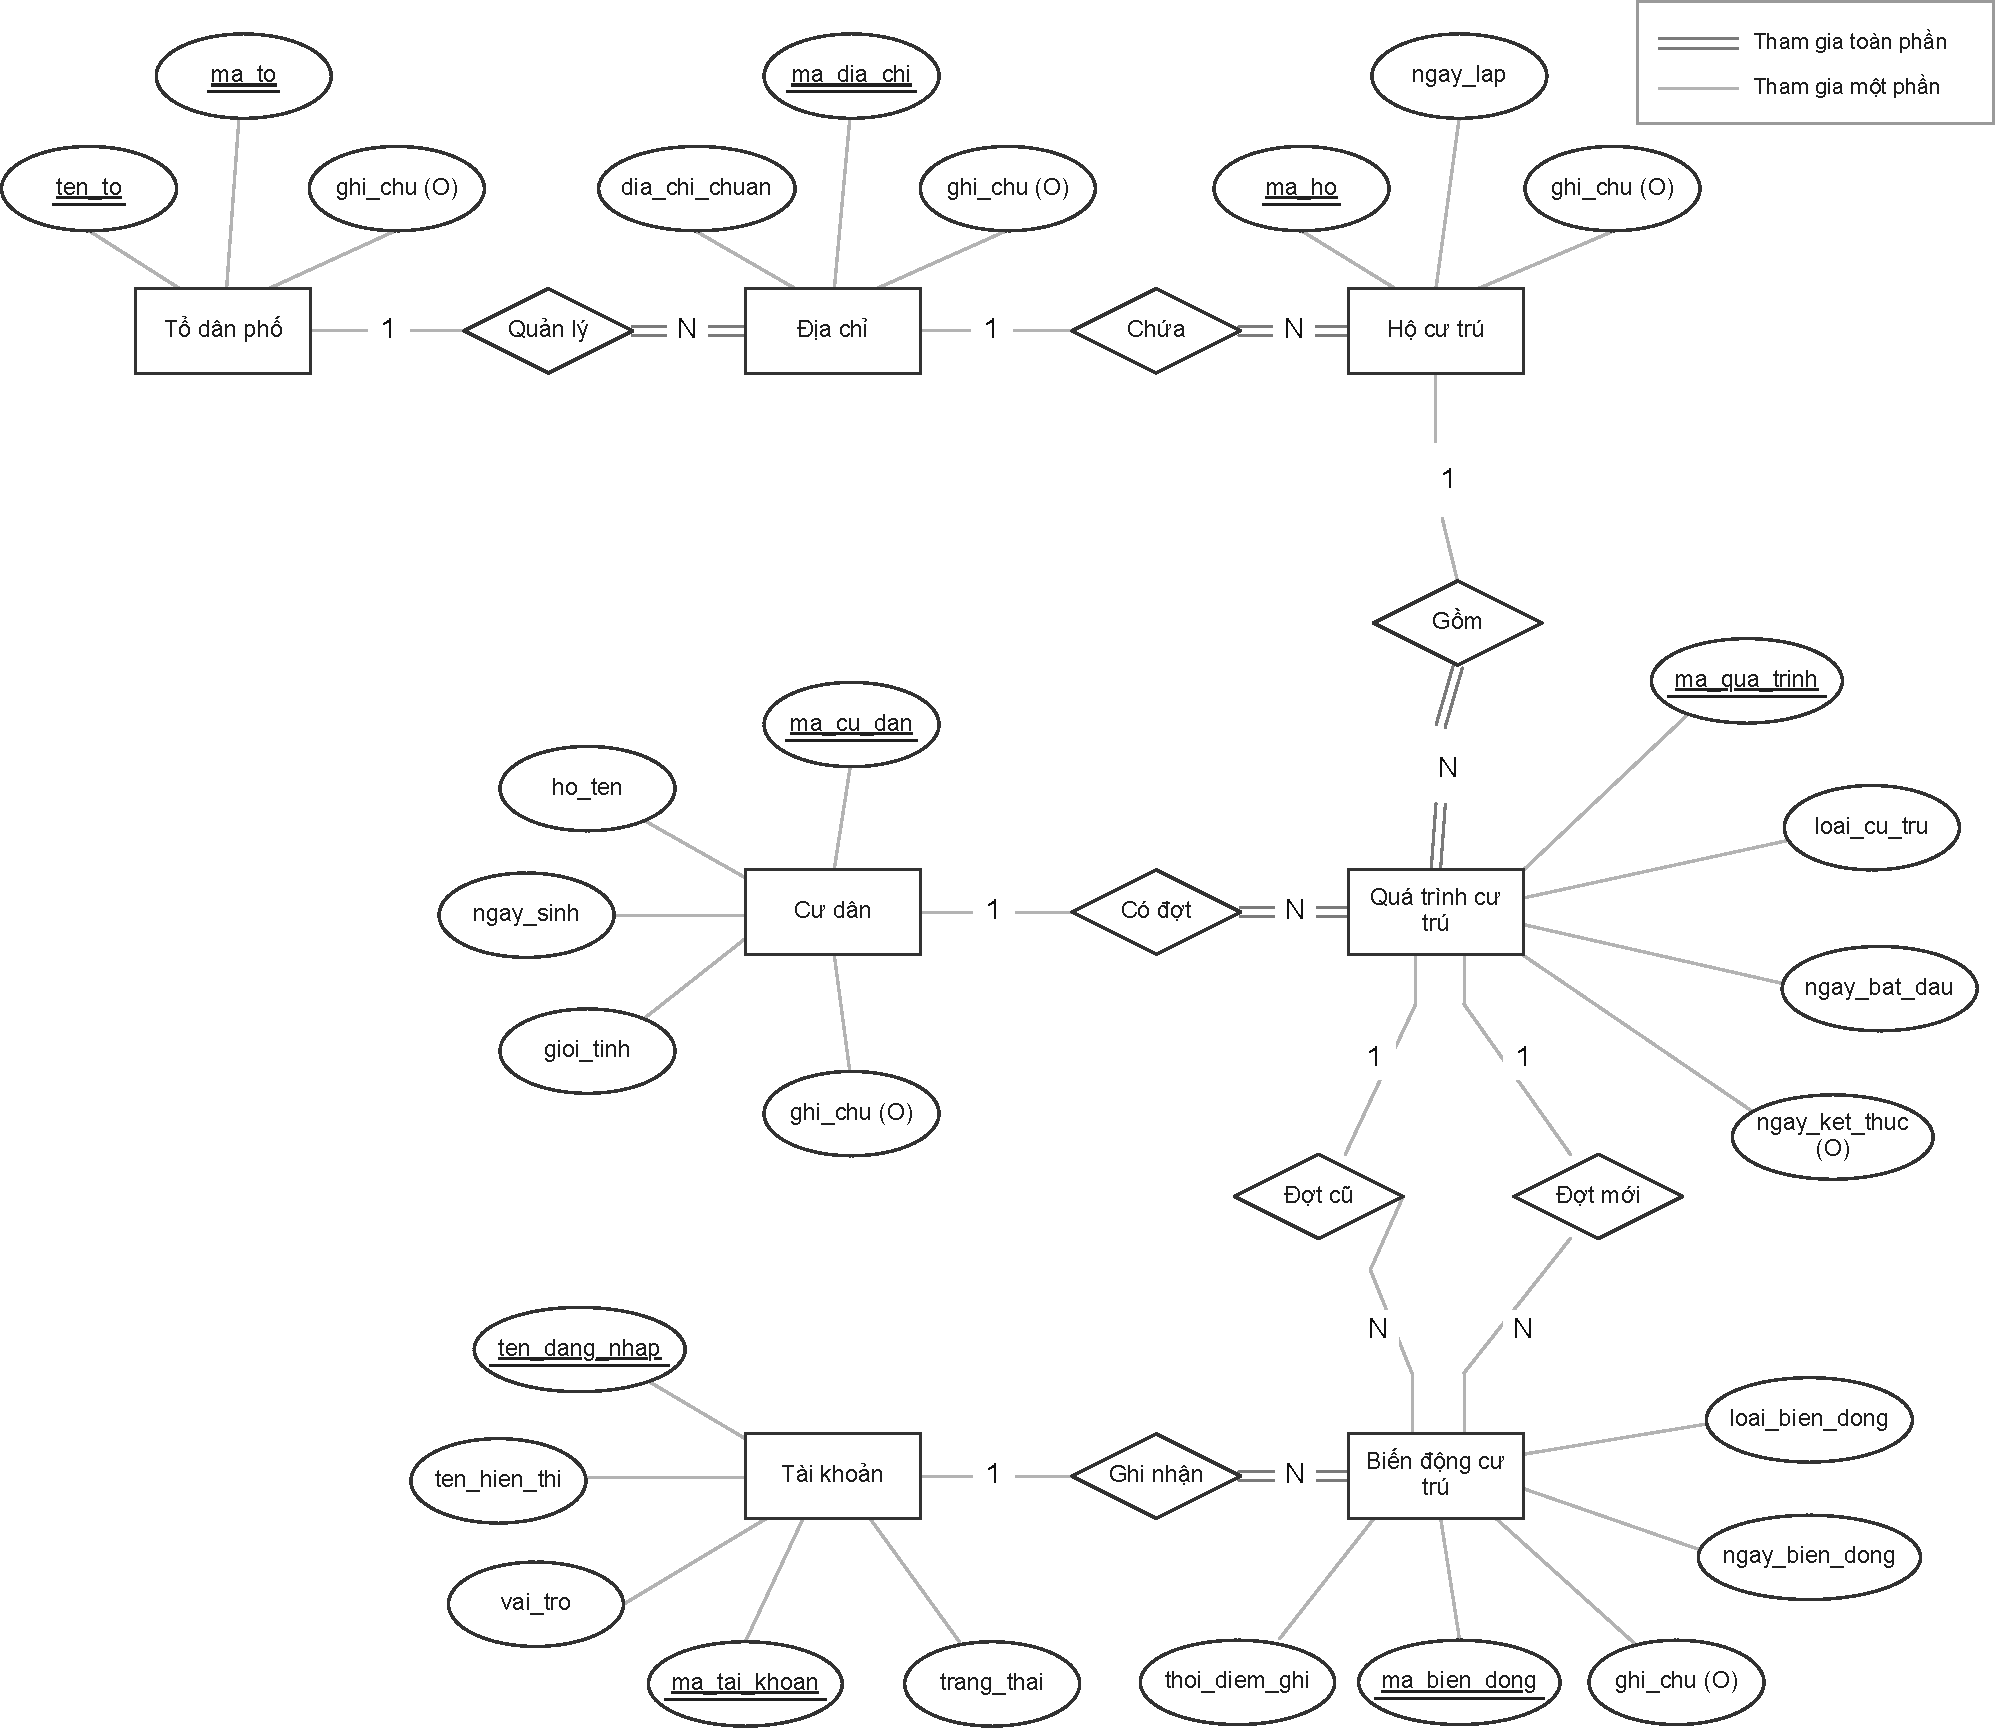
\includegraphics[width=\textwidth]{image/erd_trang_11_vector_crop.pdf}
\caption{Mô hình thực thể liên kết của hệ thống quản lý cư trú tổ dân phố}
\label{fig:erd}
\end{figure}

\subsection{Các thực thể và thuộc tính}
\label{subsec:thucthe}

\begin{table}[H]
\centering
\fontsize{12pt}{16pt}\selectfont
\renewcommand{\arraystretch}{1.15}
\begin{tabularx}{\textwidth}{|P{2.4cm}|Y|P{3.3cm}|P{3.6cm}|}
\hline
\textbf{Thực thể} & \textbf{Ý nghĩa} & \textbf{Thuộc tính khóa} & \textbf{Các thuộc tính còn lại} \\
\hline
Tổ dân phố & Một tổ dân phố thuộc phường & ma\_to; ten\_to cũng là duy nhất & ghi\_chu (O) \\
\hline
Địa chỉ & Một địa chỉ nhà nằm trong tổ, ghi theo dạng chuẩn; cặp (tổ, địa chỉ chuẩn) không trùng & ma\_dia\_chi & dia\_chi\_chuan, ghi\_chu (O) \\
\hline
Hộ cư trú & Một hộ cư trú gắn với một địa chỉ, có thể chưa phát sinh đợt cư trú & ma\_ho & ngay\_lap, ghi\_chu (O) \\
\hline
Cư dân & Một cá nhân có hồ sơ trong CSDL, có thể chưa phát sinh đợt cư trú & ma\_cu\_dan & ho\_ten, ngay\_sinh, gioi\_tinh, ghi\_chu (O) \\
\hline
Quá trình cư trú & Một đợt cư trú của một cư dân trong một hộ & ma\_qua\_trinh & loai\_cu\_tru, ngay\_bat\_dau, ngay\_ket\_thuc (O) \\
\hline
Biến động cư trú & Một lần thay đổi cư trú được cán bộ ghi nhận & ma\_bien\_dong & loai\_bien\_dong, ngay\_bien\_dong, thoi\_diem\_ghi, ghi\_chu (O) \\
\hline
Tài khoản & Tài khoản của cán bộ sử dụng hệ thống & ma\_tai\_khoan; ten\_dang\_nhap cũng là duy nhất & ten\_hien\_thi, vai\_tro, trang\_thai \\
\hline
\end{tabularx}
\caption{Các thực thể và thuộc tính}
\label{tab:thucthe}
\end{table}

Thực thể Quá trình cư trú là trung tâm của mô hình, vì nó cho biết một cư dân ở trong hộ nào, theo diện thường trú hay tạm trú và trong khoảng thời gian nào. Khi chuyển nội bộ, hệ thống đóng đợt cũ và mở đợt mới trong phường; khi chuyển ra ngoài phường, hệ thống chỉ đóng đợt cũ. Các đợt được lưu riêng để tra cứu lịch sử đã ghi nhận; việc bảo vệ chúng còn phụ thuộc quyền cập nhật và các trigger.

\subsection{Các mối liên kết}
\label{subsec:lienket}

\begin{table}[H]
\centering
\fontsize{12pt}{16pt}\selectfont
\renewcommand{\arraystretch}{1.15}
\begin{tabularx}{\textwidth}{|P{2.0cm}|P{2.5cm}|P{2.5cm}|Y|}
\hline
\textbf{Liên kết} & \textbf{Thực thể phía 1} & \textbf{Thực thể phía N} & \textbf{Giải thích} \\
\hline
Quản lý & Tổ dân phố & Địa chỉ & Một tổ quản lý nhiều địa chỉ, mỗi địa chỉ thuộc đúng một tổ \\
\hline
Chứa & Địa chỉ & Hộ cư trú & Một địa chỉ có thể có nhiều hộ, mỗi hộ ở đúng một địa chỉ \\
\hline
Gồm & Hộ cư trú & Quá trình cư trú & Một hộ gồm nhiều quá trình cư trú của các thành viên \\
\hline
Có đợt & Cư dân & Quá trình cư trú & Một cư dân có nhiều đợt cư trú theo thời gian \\
\hline
Ghi nhận & Tài khoản & Biến động cư trú & Biến động được ghi bằng đúng một tài khoản ở trạng thái hoạt động tại thời điểm ghi nhận (B14) \\
\hline
Đợt cũ & Quá trình cư trú & Biến động cư trú & Biến động làm kết thúc một quá trình (có thể không có, ví dụ chuyển đến) \\
\hline
Đợt mới & Quá trình cư trú & Biến động cư trú & Biến động mở ra một quá trình mới (có thể không có, ví dụ chuyển đi) \\
\hline
\end{tabularx}
\caption{Các mối liên kết trong mô hình}
\label{tab:lienket}
\end{table}

Giữa Quá trình cư trú và Biến động cư trú có hai liên kết song song là Đợt cũ và Đợt mới, vì một lần biến động có thể đóng một đợt cư trú và mở một đợt khác cùng lúc. Trường hợp điển hình là chuyển nội bộ: cư dân rời hộ A (đợt cũ kết thúc ngày $t-1$) và vào hộ B (đợt mới bắt đầu ngày $t$), cả hai đều gắn với cùng một bản ghi biến động.
